\section{Parallelization}
In accordance with section \ref{related_work}, the Python \code{multiprocessing} module was used to implement the parallelization of the program. Additionally, measures where taken to send as little
data as possible between processes and to avoid introducing excessive complexity to the codebase. The \code{multiprocessing.Queue} facility was chosen for communication between processes due to its
noted performance and built-in synchronization \cite{singh_2013_parallel_padpwprfmm}.

Before deciding to use the parallelized version of program, the list of filters in a file format is examined for any of the inherently serial filters
\textit{Global variable}, \textit{State variable}, or \textit{Stop processing}. If any of these are found, the
program falls back to its sequential version. Otherwise, the program carries on in accordance with figure \ref{fig:embarrassing_dag}. First, before creating any additional processes, the Header detection filter
is applied row by row until it produces a result (commonly after a few rows). Next, a (tunable) number of processes, as well as two queues are created. A number of row spans, or chunks, are then created by splitting
the rows beneath the header row into equally sized partitions. The first queue is used to transfer the data needed to process a chunk of the dataset, including the header data, the row span, and the result metadata.
In order to avoid errors and sending large objects between processes, only the primary key used to retrieve the result metadata object from the MySQL database is sent to the processes.
After this, the processes can independently retrieve the data. The second queue is used for sending the partial metrics objects for each chunk, and for indicating if a process is done processing
its data or if it encountered an error. Since all other results are written to the Cassandra database, this is the only information that needs to be sent to the main process. The queues can be
denoted the 'chunk queue' and the 'message queue', respectively.

In each of the created processes, the rows in the chunk are retrieved from the Cassandra database and a new object containing metrics for the chunk is created. The chunk is then processed as in the sequential program,
applying all filters to each row. The metrics object is updated during the processing, as in the original program. If the chunk was processed correctly, the metrics object is put on the message queue. Otherwise,
if an exception occurs, an error message is put on the queue instead. When all data in a process has finished processing, a message indicating that the process has finished its work is put on the message queue.

The main process continuously polls the message queue, and merges the partial metrics objects as they are polled from the queue. If an error message is encountered, an exception is raised on the main thread, mimicking the
behavior of the original sequential program. It also increments a counter whenever a done message is received from a process. When the counter is equal to the number of subprocesses, the main process stops waiting
for messages, and progresses with the post processing step of making the trade ID:s unique. Finally, the main process saves the result object with the corresponding merged metrics to the MySQL database. At this point,
the program has produced a finished verification result.

A simplified overview of the parallel program can be found in figure \ref{fig:parallel_program_overview}.

\begin{sidewaysfigure}[ht]
  \centering
  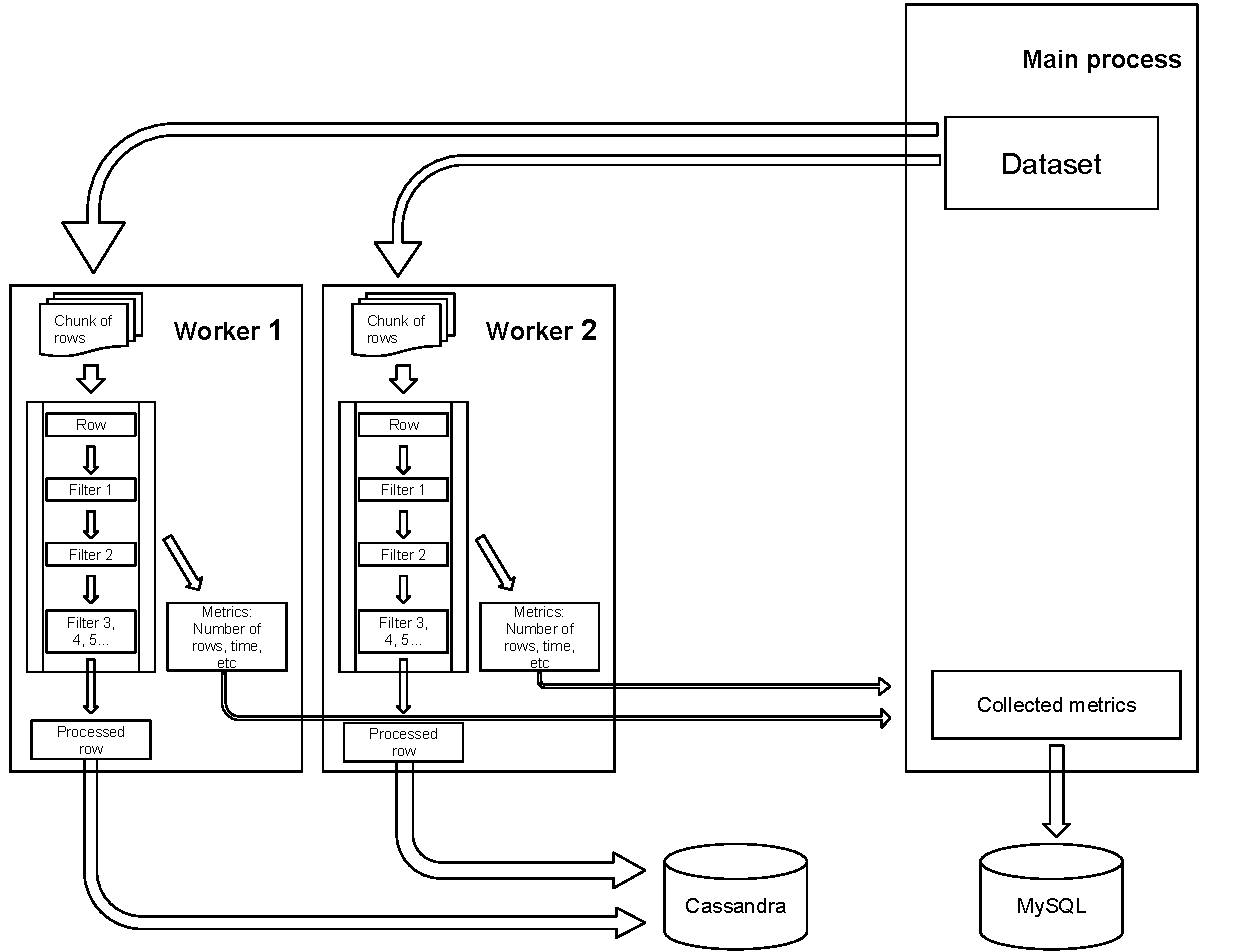
\includegraphics[width=200mm]{figures/program_overview.pdf}
  \caption[Parallel program overview.]{Parallel program overview.}
  \label{fig:parallel_program_overview}
\end{sidewaysfigure}

\section{Sources of overhead}
During the implementation of the parallel version of the program, the following possible sources of parallelization overhead where identified:

\begin{itemize}
  \item The \code{multiprocessing} module, where creating processes and transferring data between processes is costly.
  \item Less effective caching of mappings. Since the mappings cache is local to each subprocess, caches are built up individually. This results in fewer cache hits than in the sequential program, and more total work
    looking up values in the MySQL database. Hardware cache may also be affected in a similar manner.
  \item The process of making trade ID:s unique is added as an extra step after the main data processing pipeline.
  \item Because they lack built-in support for multiprocessing, the Python connections between both MySQL and Cassandra need to be restarted in the startup of each subprocess.
  \item \code{\_prepare} has to be called once for each of the workers, compared to only one call for the sequential program.
\end{itemize}
